\begin{tikzpicture}[every node/.style={inner sep=0,outer sep=0}]

	\node [anchor=north east] (imgAufbauDurchlicht) at (-0.03\textwidth,0) {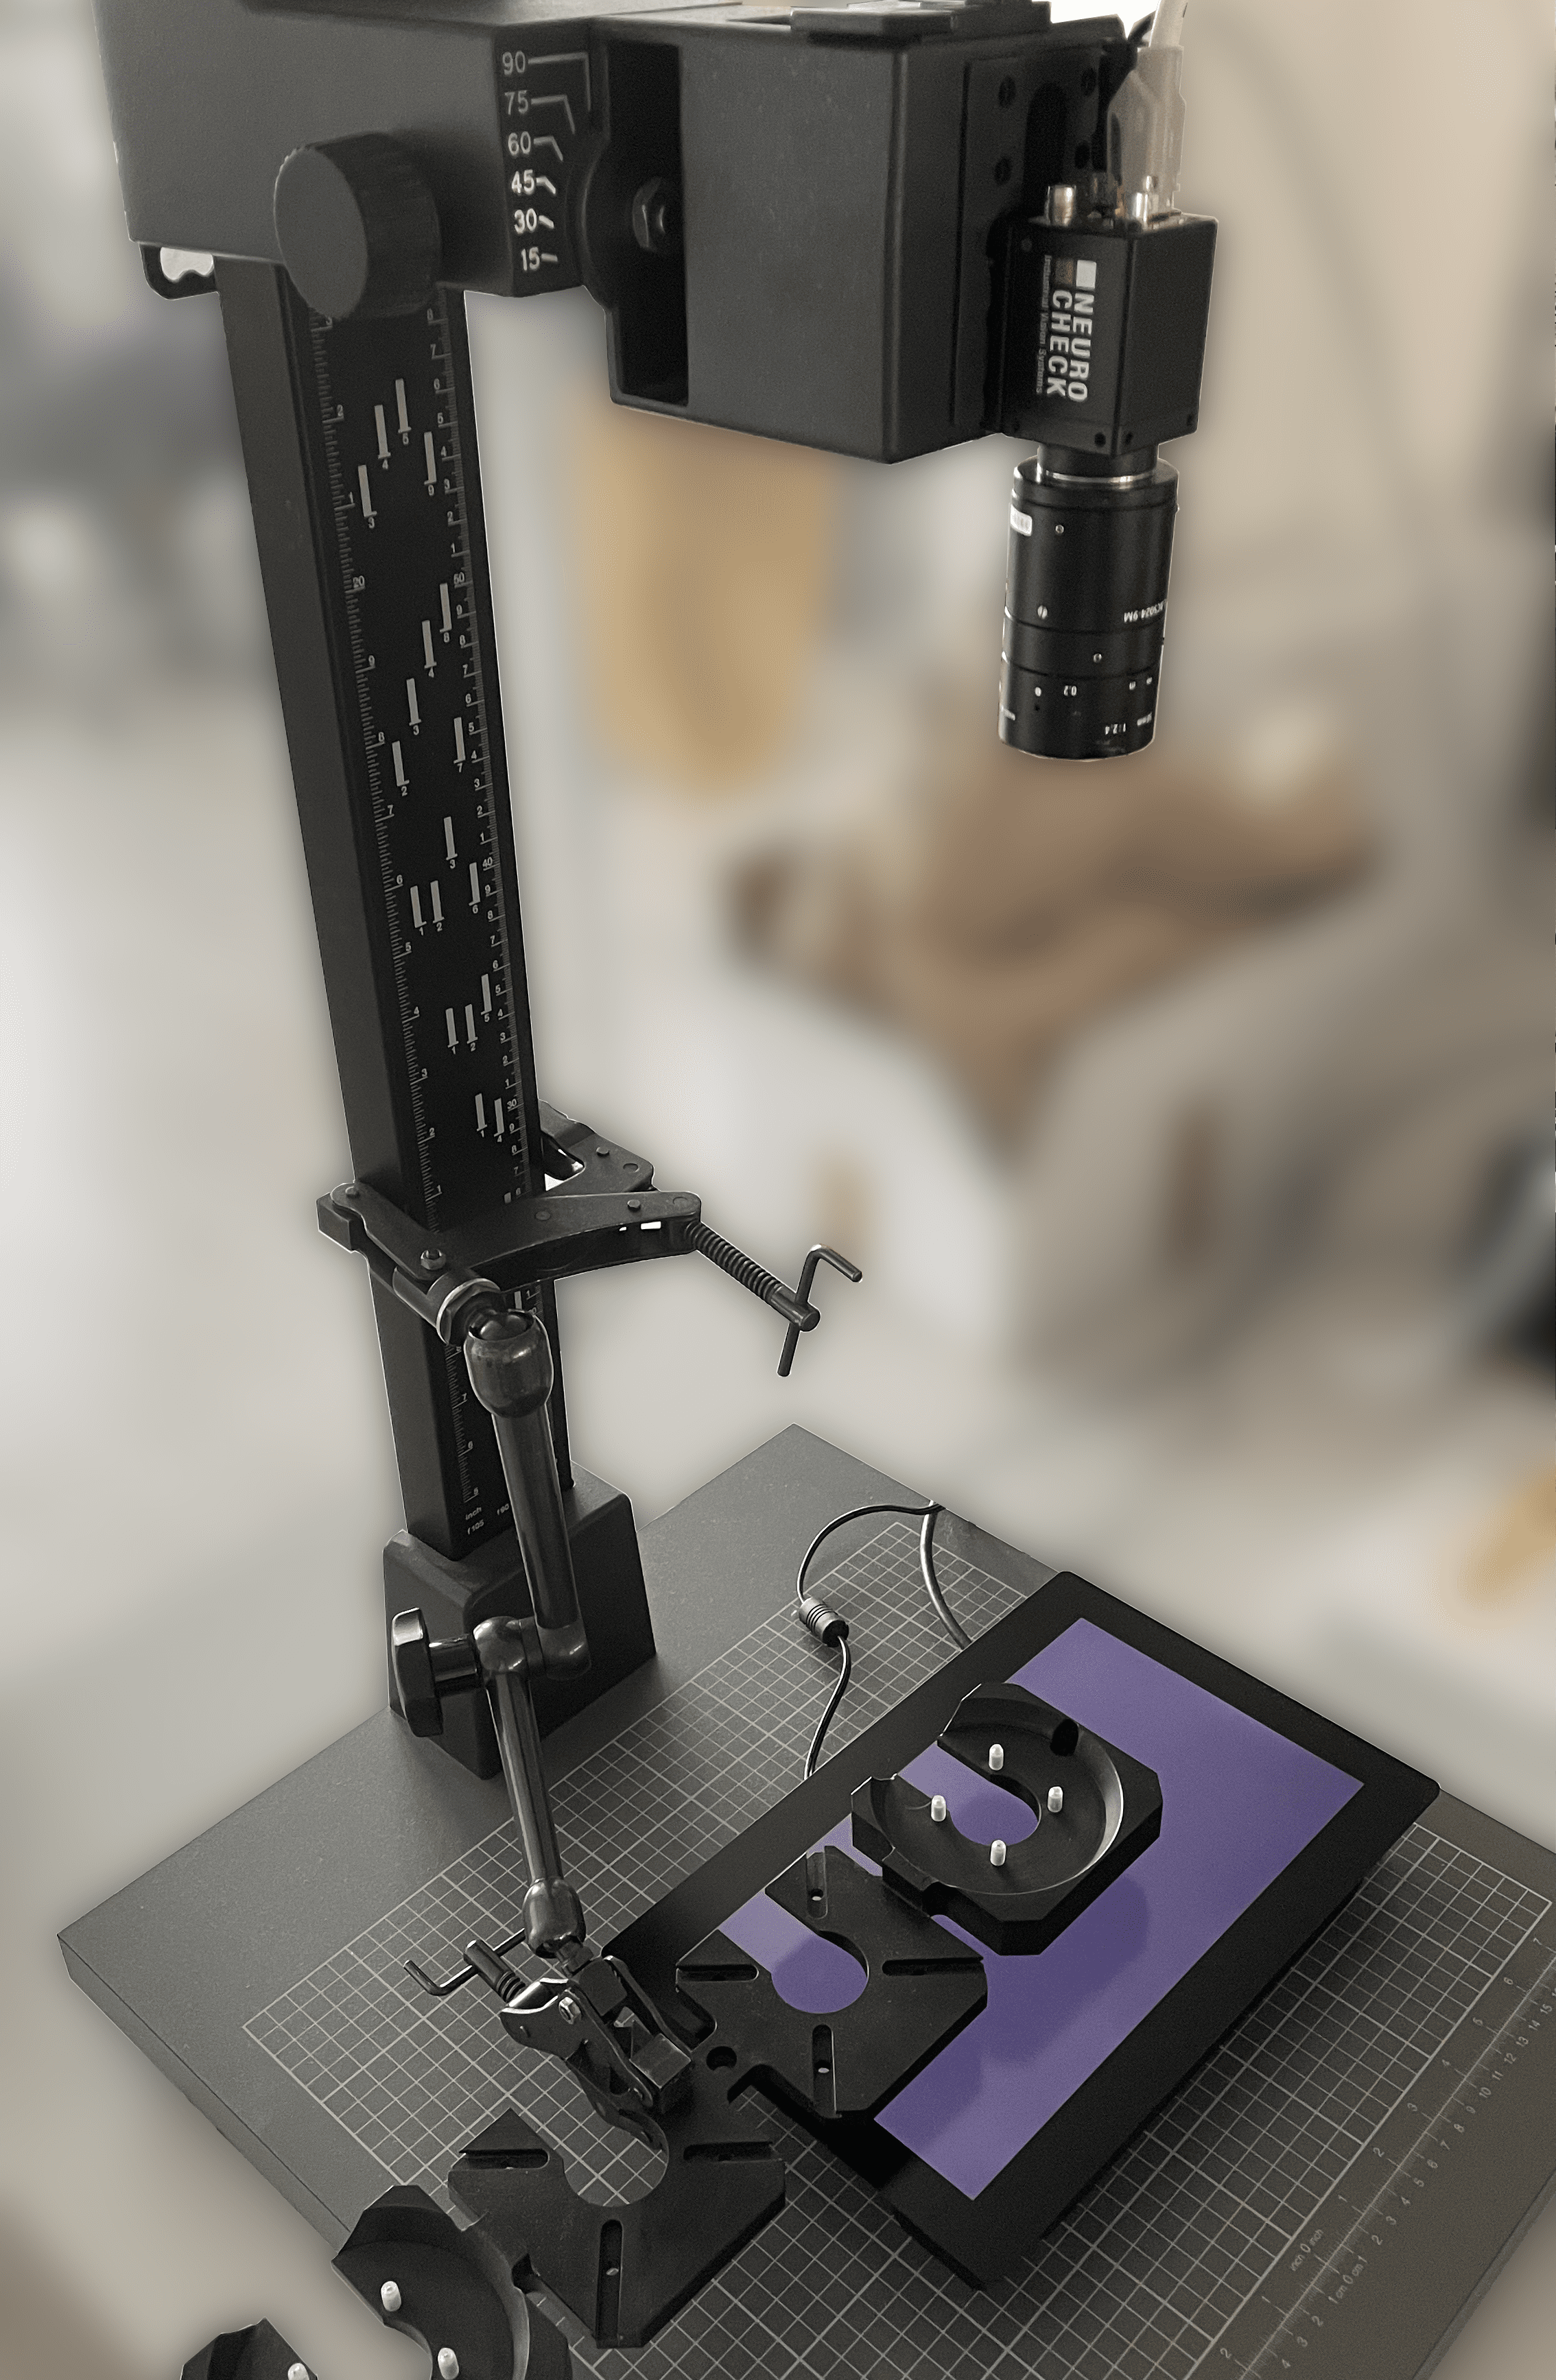
\includegraphics[width=.3\textwidth]{05_ergebnisse/figures/aufbauFotoDurchlicht}};
	\node [below=0.2cm of imgAufbauDurchlicht] {Durchlichtauswertung};
	\node [anchor=north west] (imgAufbauReflexion) at (0.03\textwidth,0) {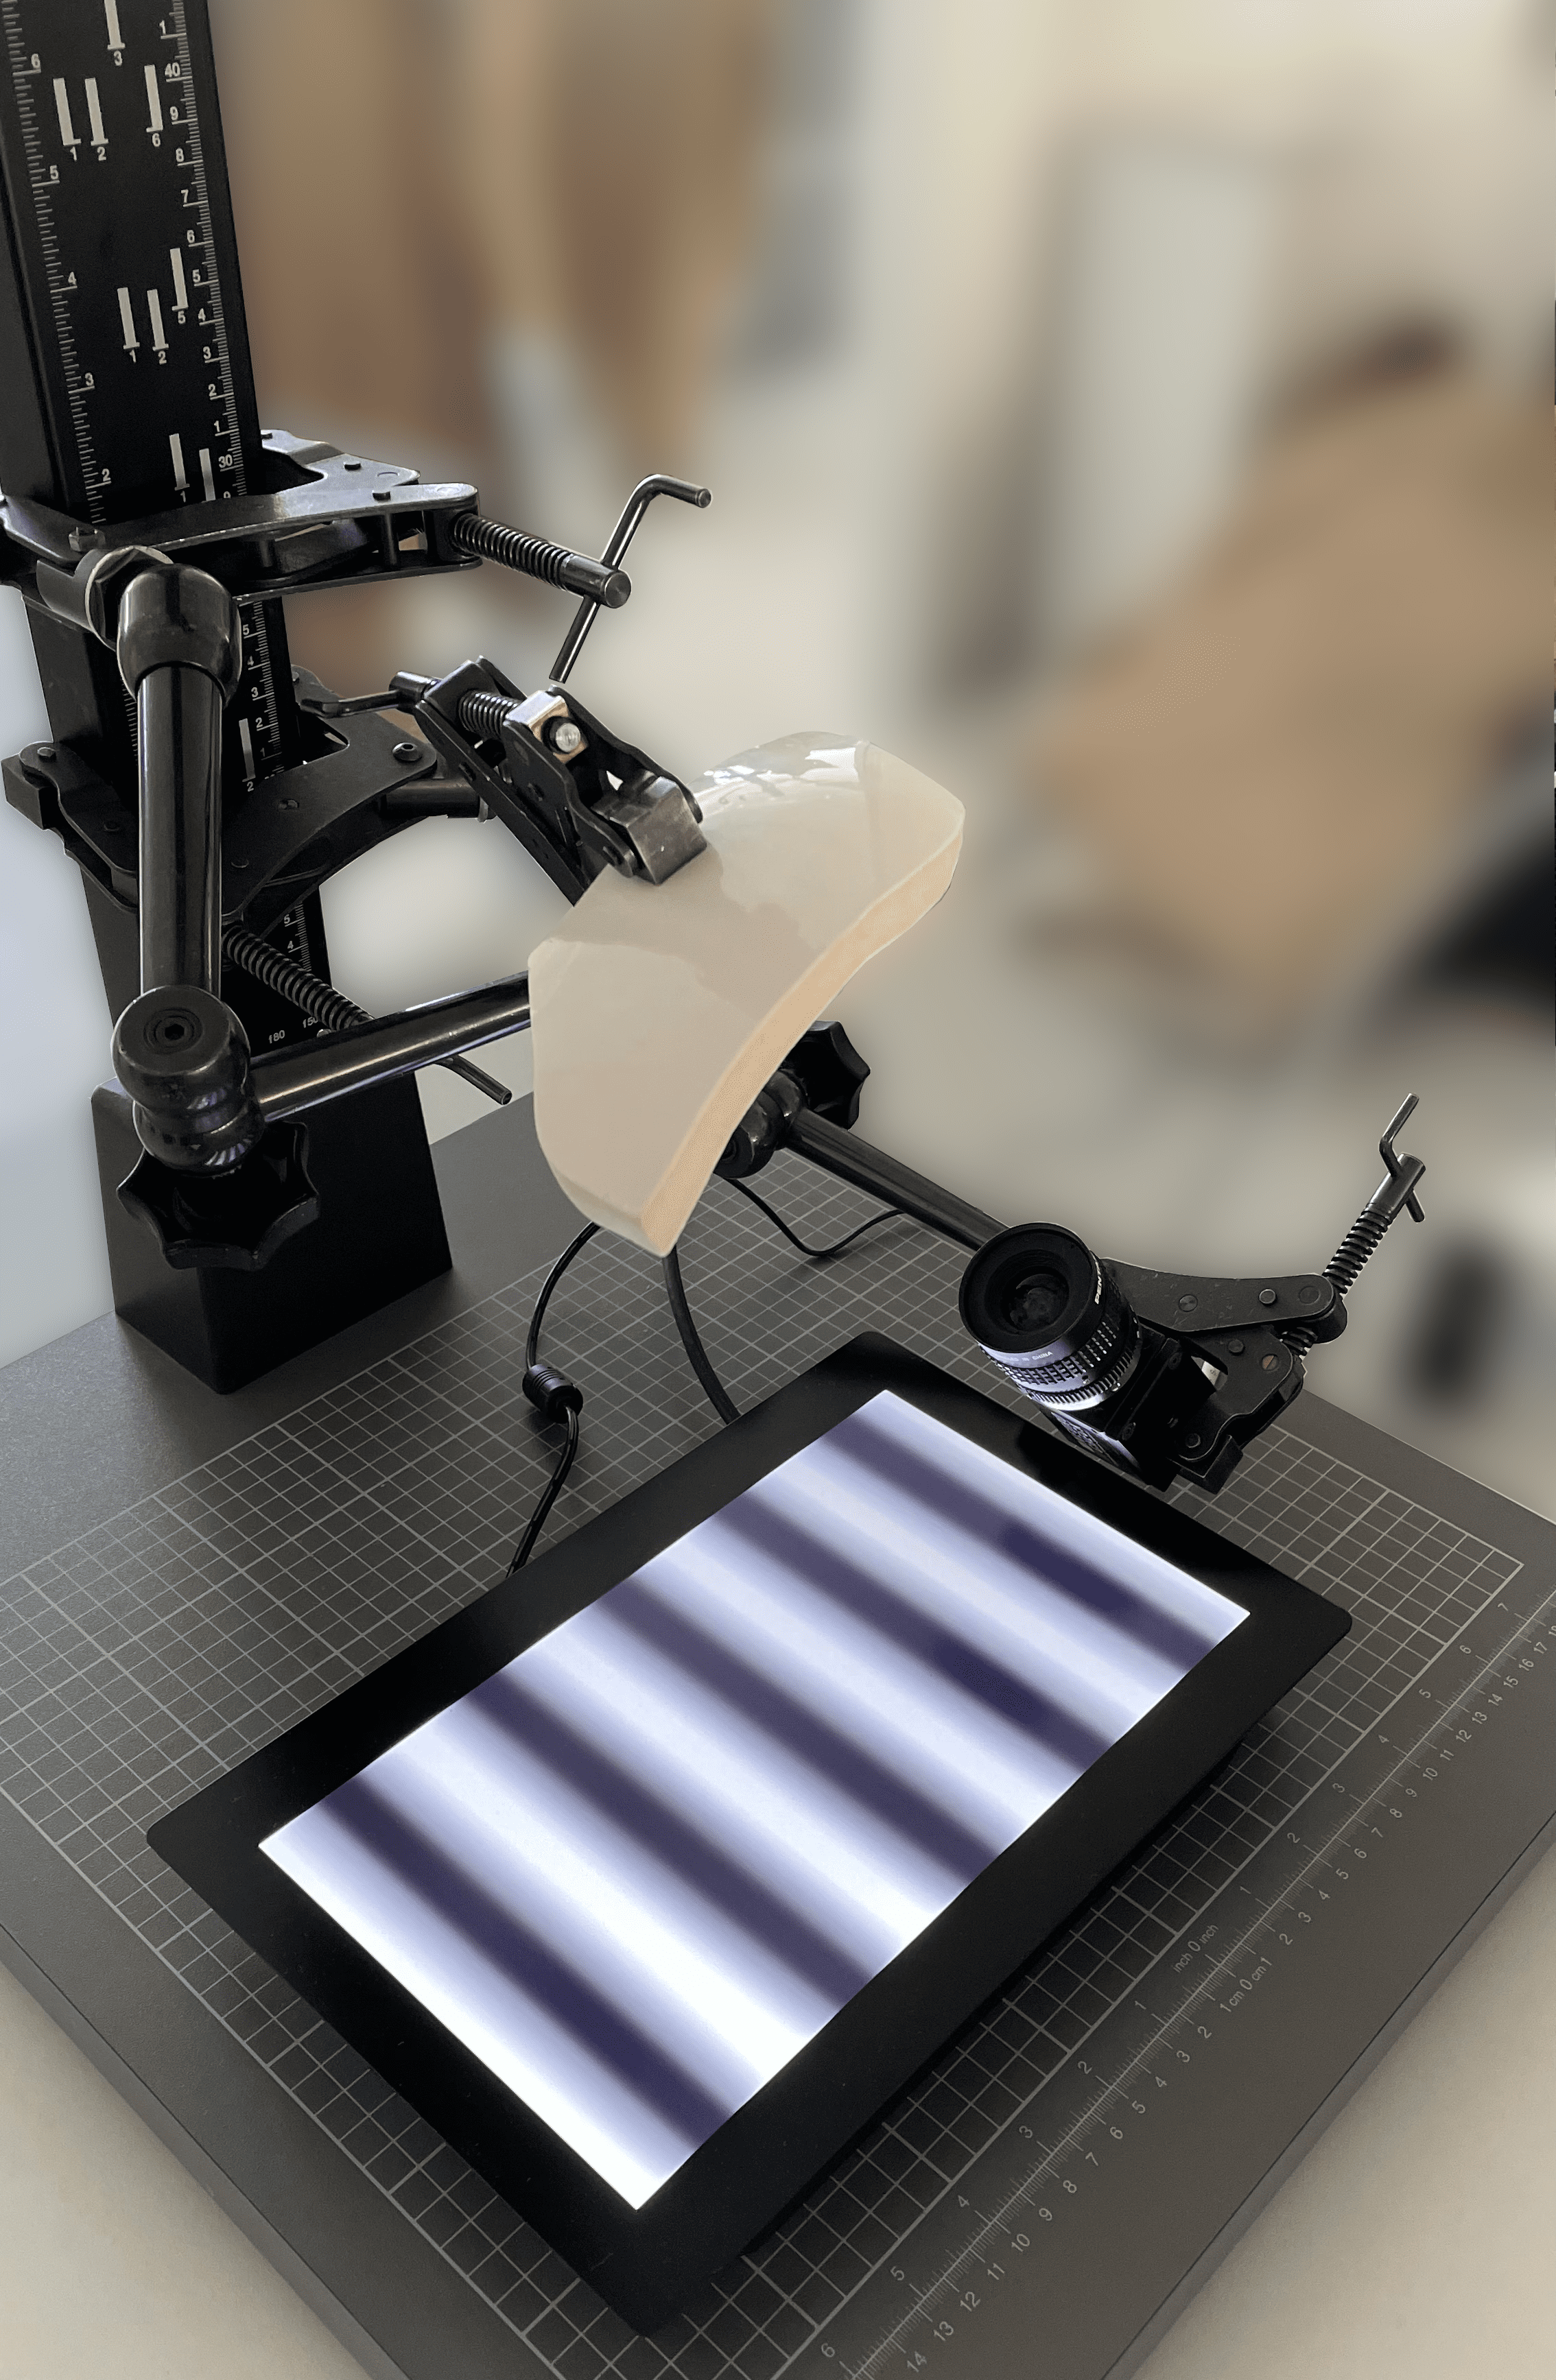
\includegraphics[width=.3\textwidth]{05_ergebnisse/figures/aufbauFotoReflexion}};
	\node [below=0.2cm of imgAufbauReflexion] {Spiegelbildauswertung};
	
\end{tikzpicture}
\caption[Verwendete Aufbauten für die Verfahren]{Verwendeten Aufbauten für die Verfahren. Links: Objektiv mit Brennweite f = 50 mm. Rechts: Objektiv mit Brennweite f = 6 mm.}